%%%%%%%%%%%%%%%%%%%%%%%%%%%%%%%%%%%%%%%%%%%%%%%%%%%%%%%%%%%%%%%%%%%%%%%%%%%%%%%%
\chapter{Finite Difference Methods}
\label{chap:fdm} % Always give a unique label
% use \chaptermark{}
% to alter or adjust the chapter heading in the running head

\abstract*{Each chapter should be preceded by an abstract (10--15 lines long) that summarizes the content. The abstract will appear \textit{online} at \url{www.SpringerLink.com} and be available with unrestricted access. This allows unregistered users to read the abstract as a teaser for the complete chapter. As a general rule the abstracts will not appear in the printed version of your book unless it is the style of your particular book or that of the series to which your book belongs.
Please use the 'starred' version of the new Springer \texttt{abstract} command for typesetting the text of the online abstracts (cf. source file of this chapter template \texttt{abstract}) and include them with the source files of your manuscript. Use the plain \texttt{abstract} command if the abstract is also to appear in the printed version of the book.}


\section{Taylor Series}
\label{sec:fdm_taylor}

% Reference Chapre and Canale
% Simple intro to Taylor Series
% Talk about truncation error

The finite difference method relies heavily on the mathematical concept of 
Taylor Series.\index{Taylor Series}  If we take a function, $f(x)$, the 
independent variable $x$ can be discretized into many points as shown in Figure \_.
If the value of the function is known at $x_{i}$, the value at $x_{i+1}$ can be
determined by a Taylor series expansion at $x_{i}$,
\begin{equation}
     f\left(x_{i+1}\right) = f\left(x_{i}\right) + f^{\prime}\left(x_{i}\right)h + 
     \frac{f^{\prime\prime}\left(x_{i}\right)}{2!}h^{2} + 
     \frac{f^{\left(3\right)}\left(x_{i}\right)}{3!}h^{3}+\cdot\cdot\cdot + 
     \frac{f^{\left(n\right)}\left(x_{i}\right)}{2!}h^{n} + \cdot\cdot\cdot
  \label{eq:fdm_taylor}
\end{equation}
In Eq. (\ref{eq:fdm_taylor}), $f^{\left(3\right)}$ represents the $n$-th derivative of 
the function and $h$ is the spacing between points, $h = x_{i+1} - x_{i}$.
\par
The expansion shown above is exact if the number of terms in the Taylor series
expansion is taken to infinity. Of course, this is not practical for computational
methods and therefore we truncate the series at a finite number of terms. The error
present caused by the truncation is known as truncation error.\index{truncation error}
Instead of representing the full Taylor expansion of a function, we will truncate
the expression after a few number of terms and repesent the truncation error with
$\mathcal{O}\left(h^{n}\right)$. In this representation of the truncation error,
$n$ represents the order of convergence.\index{order of convergence} Order of
convergence means that as the grid is refined by a factor of two for example, the
truncation error will reduce on the order of $2^{n}$. This does not imply that
one method is better than the order, just merely a concept of convergence rate
due to truncation effects. Linear convergence is when $n=1$, quadratic when $n=2$
and cubic when $n=3$. For example, if we expand a function to second order, we
would rewrite Eq. (\ref{eq:fdm_taylor}) this as
\begin{equation}
     f\left(x_{i+1}\right) = f\left(x_{i}\right) + f^{\prime}\left(x_{i}\right)h + 
     \frac{f^{\prime\prime}\left(x_{i}\right)}{2!}h^{2} + \mathcal{O}\left(h^{3}\right).
\end{equation}
As we approximate differentials, we can keep track of this truncation error to determine
order of convergence of our methods. This is one way to ensure that our discretization
method and implementation of solution algorithms are correct.

\section{Approximation of First Derivatives}
\label{sec:fdm_approx}

% Reference Chapre and Canale
% Forward, backward and central first order and second order differentials
% Simple example of Taylor expansion approximating with these approxs

There are many different approximations of differentials that can be constructed based
on Taylor series.  We will first consider the approximation of first order derivatives.
The first approximation is a \emph{first order forward difference} where we use information 
about a point just to the right, $x_{i+1}$, to infer the derivative at $x_{i}$.  If we 
perform a Taylor expansion about point $x_{i+1}$ to first order we get
\begin{equation}
     f\left(x_{i+1}\right) = f\left(x_{i}\right) + f^{\prime}\left(x_{i}\right)h + \mathcal{O}\left(h^{2}\right).
\end{equation}
This equation can be solved for the derivative of the function at $x_{i}$ 
\begin{equation}
     \boxed{f^{\prime}_{for}\left(x_{i}\right) = \frac{f\left(x_{i+1}\right) - f\left(x_{i}\right)}{h} - \mathcal{O}\left(h\right)},
  \label{eq:first_forward}
\end{equation}
where $f^{\prime}_{for}\left(x_{i}\right)$ represents the first order forward difference approximation to the derivative at
$x_{i}$.
\par
The opposite approximation is to consider a point to the left, $x_{i-1}$, to infer the
derivative at $x_{i}$, \emph{known as the first order backward difference}. Here, we take a Taylor expansion to the left,
\begin{equation}
     f\left(x_{i-1}\right) = f\left(x_{i}\right) - f^{\prime}\left(x_{i}\right)h + \mathcal{O}\left(h^{2}\right).
\end{equation}
Solving for the derivative we can arrive at
\begin{equation}
     \boxed{f^{\prime}_{bac}\left(x_{i}\right) = \frac{f\left(x_{i}\right) - f\left(x_{i-1}\right)}{h} + \mathcal{O}\left(h\right)}.
  \label{eq:first_backward}
\end{equation}
Comparing Eqs. (\ref{eq:first_forward}) and (\ref{eq:first_backward}) we see that the formulation looks the same in that it
is always the right point minus the left point in the numerator of the fraction. The only difference is the sign in the 
truncation error is reversed. Therefore, we can expect that one of these approximations will under-predict the true answer
and the other one will over-predict. Again both of these methods are first order methods.
\par 
The last simple approximation of a first derivative is a \emph{second-order central difference}. In this method we look 
at both left and right points. We can Taylor expand each of these to second order to get
\begin{eqnarray}
    f\left(x_{i+1}\right) = f\left(x_{i}\right) + f^{\prime}\left(x_{i}\right)h + \frac{f^{\prime\prime}\left(x_{i}\right)}{2!}h^{2} + \mathcal{O}\left(h^{3}\right) \\
    f\left(x_{i-1}\right) = f\left(x_{i}\right) - f^{\prime}\left(x_{i}\right)h + \frac{f^{\prime\prime}\left(x_{i}\right)}{2!}h^{2} - \mathcal{O}\left(h^{3}\right).
\end{eqnarray}
Subtracting the $x_{i-1}$ equation from the $x_{i+1}$, we are left with
\begin{equation}
    f\left(x_{i+1}\right) - f\left(x_{i-1}\right) = 2f^{\prime}\left(x_{i}\right)h  + \mathcal{O}\left(h^{3}\right).
\end{equation}
Solving for the derivative at $x_{i}$ we arrive at the second order central difference approximation
\begin{equation}
    \boxed{f^{\prime}_{cen}\left(x_{i}\right) = \frac{f\left(x_{i+1}\right) - f\left(x_{i-1}\right)}{2h} - \mathcal{O}\left(h^{2}\right)}.
\end{equation}
From the resulting expression, this approximation method does not depend on the value of the function at $x_{i}$ and that
the scheme is second order convergent.
\par
\begin{figure}[t]
\sidecaption[t]
\scalebox{0.5}{% This file was created by matlab2tikz v0.1.4.
% Copyright (c) 2008--2011, Nico Schlömer <nico.schloemer@gmail.com>
% All rights reserved.
% 
% The latest updates can be retrieved from
%   http://www.mathworks.com/matlabcentral/fileexchange/22022-matlab2tikz
% where you can also make suggestions and rate matlab2tikz.
% 
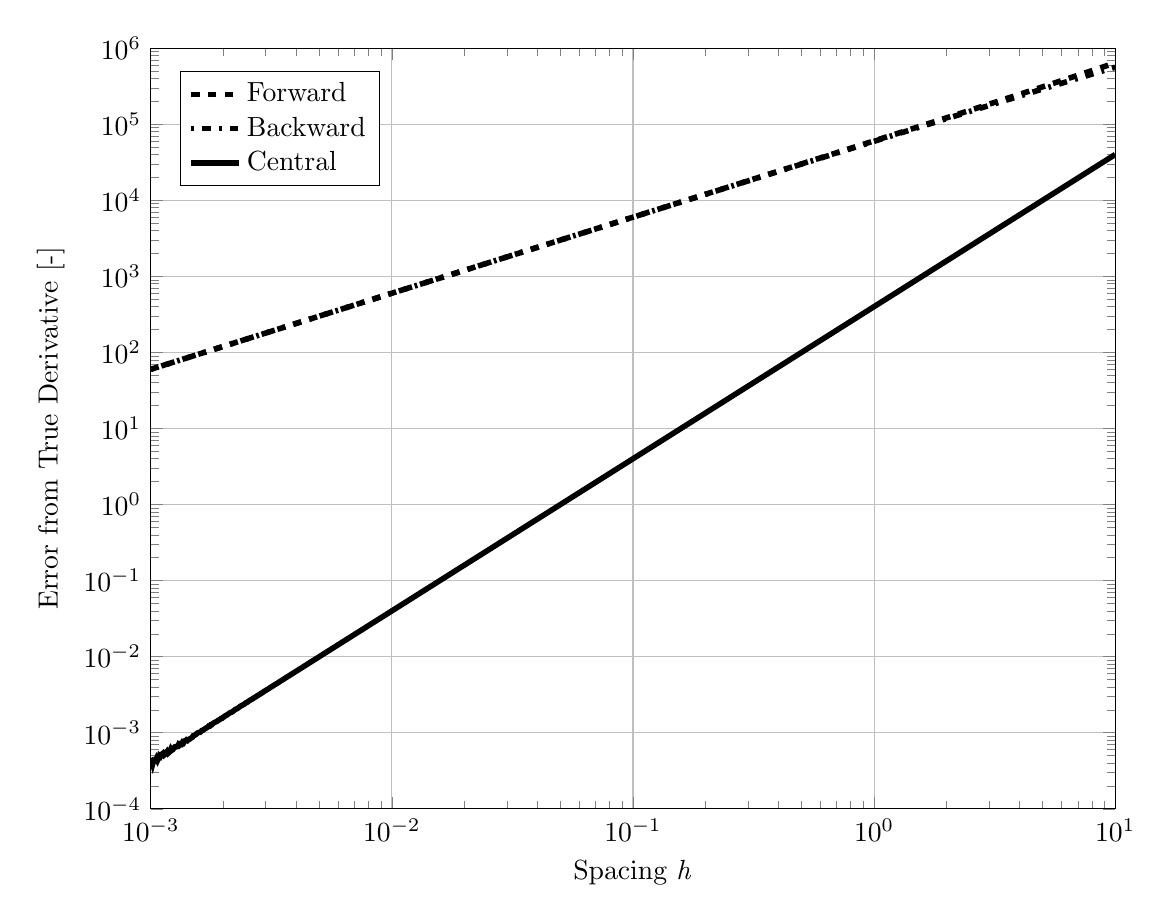
\begin{tikzpicture}

\begin{loglogaxis}[%
scale only axis,
width=4.82222in,
height=3.80333in,
xmin=0.001, xmax=10,
ymin=0.0001, ymax=1e+06,
xminorticks=true,
yminorticks=true,
xlabel={Spacing \emph{h}},
ylabel={Error from True Derivative [-]},
xmajorgrids,
ymajorgrids,
legend entries={Forward,Backward,Central},
legend style={at={(0.03,0.97)},anchor=north west,nodes=right}]
\addplot [
color=black,
dashed,
line width=2.0pt
]
coordinates{
 (0.001,60.0004)(0.00100926,60.5562)(0.00101861,61.117)(0.00102804,61.6831)(0.00103757,62.2544)(0.00104718,62.831)(0.00105688,63.413)(0.00106666,64.0003)(0.00107654,64.5931)(0.00108652,65.1914)(0.00109658,65.7952)(0.00110674,66.4047)(0.00111699,67.0197)(0.00112733,67.6405)(0.00113777,68.267)(0.00114831,68.8993)(0.00115895,69.5374)(0.00116968,70.1815)(0.00118052,70.8315)(0.00119145,71.4876)(0.00120249,72.1497)(0.00121362,72.818)(0.00122486,73.4925)(0.00123621,74.1732)(0.00124766,74.8602)(0.00125922,75.5536)(0.00127088,76.2534)(0.00128265,76.9596)(0.00129453,77.6725)(0.00130652,78.3919)(0.00131862,79.118)(0.00133083,79.8508)(0.00134316,80.5904)(0.0013556,81.3369)(0.00136816,82.0902)(0.00138083,82.8506)(0.00139362,83.6179)(0.00140653,84.3924)(0.00141955,85.1741)(0.0014327,85.963)(0.00144597,86.7592)(0.00145937,87.5628)(0.00147288,88.3738)(0.00148652,89.1924)(0.00150029,90.0185)(0.00151419,90.8523)(0.00152821,91.6938)(0.00154237,92.5431)(0.00155665,93.4002)(0.00157107,94.2653)(0.00158562,95.1384)(0.00160031,96.0196)(0.00161513,96.909)(0.00163009,97.8066)(0.00164519,98.7125)(0.00166043,99.6268)(0.00167581,100.55)(0.00169133,101.481)(0.00170699,102.421)(0.00172281,103.37)(0.00173876,104.327)(0.00175487,105.293)(0.00177112,106.269)(0.00178753,107.253)(0.00180408,108.246)(0.00182079,109.249)(0.00183766,110.261)(0.00185468,111.282)(0.00187186,112.313)(0.00188919,113.353)(0.00190669,114.403)(0.00192435,115.463)(0.00194217,116.532)(0.00196016,117.611)(0.00197832,118.701)(0.00199664,119.8)(0.00201514,120.91)(0.0020338,122.03)(0.00205264,123.16)(0.00207165,124.301)(0.00209084,125.452)(0.0021102,126.614)(0.00212975,127.787)(0.00214947,128.97)(0.00216938,130.165)(0.00218948,131.371)(0.00220976,132.587)(0.00223022,133.815)(0.00225088,135.055)(0.00227173,136.306)(0.00229277,137.568)(0.00231401,138.842)(0.00233544,140.128)(0.00235707,141.426)(0.0023789,142.736)(0.00240093,144.058)(0.00242317,145.393)(0.00244562,146.739)(0.00246827,148.099)(0.00249113,149.47)(0.0025142,150.855)(0.00253749,152.252)(0.00256099,153.662)(0.00258471,155.085)(0.00260865,156.522)(0.00263282,157.972)(0.0026572,159.435)(0.00268181,160.912)(0.00270665,162.402)(0.00273172,163.906)(0.00275702,165.424)(0.00278256,166.957)(0.00280833,168.503)(0.00283434,170.064)(0.0028606,171.639)(0.00288709,173.229)(0.00291383,174.833)(0.00294082,176.453)(0.00296806,178.087)(0.00299555,179.737)(0.00302329,181.401)(0.0030513,183.082)(0.00307956,184.777)(0.00310808,186.489)(0.00313687,188.216)(0.00316592,189.959)(0.00319525,191.719)(0.00322484,193.495)(0.00325471,195.287)(0.00328486,197.096)(0.00331528,198.921)(0.00334599,200.764)(0.00337698,202.623)(0.00340826,204.5)(0.00343983,206.394)(0.00347169,208.306)(0.00350384,210.235)(0.0035363,212.183)(0.00356905,214.148)(0.00360211,216.132)(0.00363547,218.133)(0.00366914,220.154)(0.00370313,222.193)(0.00373743,224.251)(0.00377204,226.328)(0.00380698,228.425)(0.00384224,230.54)(0.00387783,232.676)(0.00391375,234.831)(0.00395,237.006)(0.00398658,239.201)(0.00402351,241.417)(0.00406077,243.653)(0.00409838,245.91)(0.00413634,248.187)(0.00417466,250.486)(0.00421332,252.806)(0.00425235,255.148)(0.00429173,257.511)(0.00433148,259.897)(0.0043716,262.304)(0.00441209,264.733)(0.00445296,267.185)(0.0044942,269.66)(0.00453583,272.158)(0.00457784,274.679)(0.00462024,277.223)(0.00466303,279.791)(0.00470622,282.382)(0.00474981,284.998)(0.00479381,287.638)(0.00483821,290.302)(0.00488302,292.991)(0.00492825,295.705)(0.0049739,298.444)(0.00501997,301.208)(0.00506646,303.998)(0.00511339,306.814)(0.00516075,309.656)(0.00520855,312.524)(0.00525679,315.419)(0.00530548,318.34)(0.00535462,321.289)(0.00540422,324.265)(0.00545427,327.268)(0.00550479,330.3)(0.00555578,333.359)(0.00560723,336.447)(0.00565917,339.563)(0.00571159,342.708)(0.00576449,345.883)(0.00581788,349.086)(0.00587177,352.32)(0.00592615,355.583)(0.00598104,358.877)(0.00603644,362.201)(0.00609235,365.556)(0.00614878,368.942)(0.00620573,372.359)(0.00626321,375.808)(0.00632122,379.289)(0.00637977,382.802)(0.00643886,386.348)(0.0064985,389.927)(0.00655869,393.538)(0.00661943,397.184)(0.00668074,400.862)(0.00674262,404.576)(0.00680507,408.323)(0.0068681,412.105)(0.00693172,415.922)(0.00699592,419.775)(0.00706072,423.663)(0.00712612,427.587)(0.00719212,431.548)(0.00725873,435.545)(0.00732597,439.579)(0.00739382,443.651)(0.0074623,447.76)(0.00753142,451.908)(0.00760118,456.094)(0.00767158,460.318)(0.00774264,464.582)(0.00781435,468.885)(0.00788673,473.229)(0.00795978,477.612)(0.0080335,482.036)(0.00810791,486.501)(0.00818301,491.007)(0.0082588,495.555)(0.00833529,500.145)(0.0084125,504.778)(0.00849042,509.454)(0.00856906,514.173)(0.00864842,518.935)(0.00872853,523.742)(0.00880937,528.593)(0.00889097,533.49)(0.00897332,538.431)(0.00905643,543.419)(0.00914031,548.452)(0.00922497,553.532)(0.00931041,558.659)(0.00939665,563.834)(0.00948368,569.057)(0.00957152,574.328)(0.00966017,579.648)(0.00974965,585.017)(0.00983995,590.436)(0.00993109,595.905)(0.0100231,601.425)(0.0101159,606.996)(0.0102096,612.618)(0.0103042,618.293)(0.0103996,624.02)(0.0104959,629.8)(0.0105931,635.634)(0.0106913,641.522)(0.0107903,647.464)(0.0108902,653.461)(0.0109911,659.514)(0.0110929,665.623)(0.0111956,671.789)(0.0112993,678.011)(0.011404,684.292)(0.0115096,690.63)(0.0116162,697.028)(0.0117238,703.484)(0.0118324,710)(0.011942,716.577)(0.0120526,723.215)(0.0121642,729.914)(0.0122769,736.675)(0.0123906,743.499)(0.0125054,750.386)(0.0126212,757.337)(0.0127381,764.352)(0.0128561,771.432)(0.0129752,778.578)(0.0130954,785.79)(0.0132166,793.068)(0.0133391,800.415)(0.0134626,807.829)(0.0135873,815.312)(0.0137131,822.864)(0.0138402,830.486)(0.0139684,838.179)(0.0140977,845.943)(0.0142283,853.779)(0.0143601,861.688)(0.0144931,869.67)(0.0146273,877.726)(0.0147628,885.856)(0.0148996,894.062)(0.0150376,902.344)(0.0151768,910.702)(0.0153174,919.138)(0.0154593,927.652)(0.0156025,936.245)(0.015747,944.918)(0.0158928,953.671)(0.01604,962.505)(0.0161886,971.421)(0.0163385,980.419)(0.0164899,989.501)(0.0166426,998.667)(0.0167967,1007.92)(0.0169523,1017.25)(0.0171093,1026.68)(0.0172678,1036.19)(0.0174277,1045.79)(0.0175892,1055.47)(0.0177521,1065.25)(0.0179165,1075.12)(0.0180824,1085.08)(0.0182499,1095.13)(0.018419,1105.27)(0.0185896,1115.51)(0.0187617,1125.85)(0.0189355,1136.27)(0.0191109,1146.8)(0.0192879,1157.42)(0.0194666,1168.15)(0.0196469,1178.97)(0.0198288,1189.89)(0.0200125,1200.91)(0.0201979,1212.03)(0.0203849,1223.26)(0.0205737,1234.59)(0.0207643,1246.03)(0.0209566,1257.57)(0.0211507,1269.22)(0.0213466,1280.98)(0.0215443,1292.85)(0.0217439,1304.82)(0.0219453,1316.91)(0.0221486,1329.11)(0.0223537,1341.42)(0.0225607,1353.85)(0.0227697,1366.39)(0.0229806,1379.05)(0.0231935,1391.82)(0.0234083,1404.72)(0.0236251,1417.73)(0.0238439,1430.86)(0.0240648,1444.12)(0.0242876,1457.49)(0.0245126,1471)(0.0247396,1484.62)(0.0249688,1498.38)(0.0252,1512.26)(0.0254335,1526.27)(0.025669,1540.41)(0.0259068,1554.68)(0.0261467,1569.08)(0.0263889,1583.61)(0.0266333,1598.28)(0.02688,1613.09)(0.027129,1628.03)(0.0273803,1643.11)(0.0276339,1658.34)(0.0278898,1673.7)(0.0281481,1689.2)(0.0284088,1704.85)(0.028672,1720.65)(0.0289375,1736.59)(0.0292056,1752.67)(0.0294761,1768.91)(0.0297491,1785.3)(0.0300246,1801.84)(0.0303027,1818.53)(0.0305834,1835.38)(0.0308666,1852.38)(0.0311525,1869.54)(0.0314411,1886.86)(0.0317323,1904.34)(0.0320262,1921.98)(0.0323228,1939.79)(0.0326222,1957.76)(0.0329244,1975.9)(0.0332293,1994.2)(0.0335371,2012.68)(0.0338477,2031.32)(0.0341612,2050.14)(0.0344776,2069.13)(0.034797,2088.3)(0.0351193,2107.65)(0.0354446,2127.18)(0.0357729,2146.88)(0.0361042,2166.77)(0.0364386,2186.85)(0.0367761,2207.11)(0.0371167,2227.55)(0.0374605,2248.19)(0.0378075,2269.02)(0.0381576,2290.04)(0.0385111,2311.26)(0.0388678,2332.67)(0.0392278,2354.28)(0.0395911,2376.09)(0.0399578,2398.11)(0.0403279,2420.32)(0.0407014,2442.75)(0.0410784,2465.38)(0.0414589,2488.22)(0.0418429,2511.27)(0.0422304,2534.54)(0.0426216,2558.02)(0.0430164,2581.72)(0.0434148,2605.64)(0.0438169,2629.78)(0.0442227,2654.15)(0.0446323,2678.74)(0.0450457,2703.56)(0.045463,2728.6)(0.045884,2753.88)(0.046309,2779.4)(0.046738,2805.15)(0.0471708,2831.14)(0.0476078,2857.37)(0.0480487,2883.85)(0.0484937,2910.57)(0.0489429,2937.53)(0.0493962,2964.75)(0.0498537,2992.22)(0.0503155,3019.94)(0.0507815,3047.92)(0.0512519,3076.16)(0.0517266,3104.66)(0.0522057,3133.43)(0.0526892,3162.46)(0.0531772,3191.77)(0.0536698,3221.34)(0.0541669,3251.19)(0.0546686,3281.31)(0.0551749,3311.71)(0.055686,3342.4)(0.0562017,3373.37)(0.0567223,3404.62)(0.0572477,3436.17)(0.0577779,3468.01)(0.0583131,3500.14)(0.0588532,3532.58)(0.0593983,3565.31)(0.0599484,3598.34)(0.0605037,3631.69)(0.0610641,3665.34)(0.0616297,3699.3)(0.0622005,3733.58)(0.0627766,3768.17)(0.063358,3803.09)(0.0639449,3838.33)(0.0645372,3873.9)(0.0651349,3909.79)(0.0657382,3946.02)(0.0663471,3982.59)(0.0669616,4019.49)(0.0675818,4056.74)(0.0682078,4094.33)(0.0688395,4132.27)(0.0694771,4170.56)(0.0701206,4209.21)(0.0707701,4248.21)(0.0714256,4287.58)(0.0720872,4327.31)(0.0727548,4367.41)(0.0734287,4407.88)(0.0741088,4448.73)(0.0747952,4489.95)(0.075488,4531.56)(0.0761872,4573.55)(0.0768928,4615.94)(0.077605,4658.71)(0.0783238,4701.88)(0.0790493,4745.46)(0.0797814,4789.43)(0.0805204,4833.82)(0.0812662,4878.61)(0.0820189,4923.83)(0.0827786,4969.46)(0.0835453,5015.51)(0.0843191,5061.99)(0.0851001,5108.9)(0.0858883,5156.25)(0.0866838,5204.03)(0.0874867,5252.26)(0.088297,5300.94)(0.0891148,5350.07)(0.0899402,5399.65)(0.0907733,5449.69)(0.091614,5500.2)(0.0924626,5551.17)(0.093319,5602.62)(0.0941833,5654.55)(0.0950557,5706.95)(0.0959361,5759.85)(0.0968247,5813.23)(0.0977215,5867.11)(0.0986266,5921.49)(0.0995401,5976.37)(0.100462,6031.76)(0.101393,6087.67)(0.102332,6144.09)(0.103279,6201.04)(0.104236,6258.51)(0.105202,6316.52)(0.106176,6375.07)(0.107159,6434.15)(0.108152,6493.79)(0.109154,6553.98)(0.110165,6614.73)(0.111185,6676.04)(0.112215,6737.92)(0.113254,6800.38)(0.114303,6863.41)(0.115362,6927.03)(0.11643,6991.24)(0.117509,7056.05)(0.118597,7121.45)(0.119696,7187.47)(0.120804,7254.09)(0.121923,7321.34)(0.123052,7389.2)(0.124192,7457.7)(0.125342,7526.83)(0.126503,7596.61)(0.127675,7667.03)(0.128858,7738.1)(0.130051,7809.84)(0.131256,7882.23)(0.132471,7955.31)(0.133698,8029.05)(0.134937,8103.49)(0.136187,8178.61)(0.137448,8254.43)(0.138721,8330.96)(0.140006,8408.19)(0.141303,8486.15)(0.142611,8564.82)(0.143932,8644.23)(0.145265,8724.37)(0.146611,8805.25)(0.147969,8886.89)(0.149339,8969.28)(0.150723,9052.44)(0.152119,9136.37)(0.153528,9221.08)(0.15495,9306.58)(0.156385,9392.87)(0.157833,9479.96)(0.159295,9567.86)(0.16077,9656.57)(0.16226,9746.11)(0.163762,9836.48)(0.165279,9927.68)(0.16681,10019.7)(0.168355,10112.6)(0.169914,10206.4)(0.171488,10301.1)(0.173077,10396.6)(0.17468,10493)(0.176298,10590.3)(0.17793,10688.5)(0.179578,10787.6)(0.181242,10887.7)(0.18292,10988.6)(0.184615,11090.5)(0.186325,11193.4)(0.18805,11297.2)(0.189792,11401.9)(0.19155,11507.7)(0.193324,11614.4)(0.195115,11722.1)(0.196922,11830.8)(0.198746,11940.6)(0.200587,12051.3)(0.202445,12163.1)(0.20432,12275.9)(0.206212,12389.7)(0.208122,12504.7)(0.21005,12620.6)(0.211995,12737.7)(0.213959,12855.9)(0.215941,12975.1)(0.217941,13095.5)(0.219959,13216.9)(0.221997,13339.5)(0.224053,13463.3)(0.226128,13588.1)(0.228222,13714.2)(0.230336,13841.4)(0.23247,13969.8)(0.234623,14099.4)(0.236796,14230.2)(0.238989,14362.2)(0.241203,14495.5)(0.243437,14629.9)(0.245692,14765.7)(0.247967,14902.6)(0.250264,15040.9)(0.252582,15180.5)(0.254921,15321.3)(0.257283,15463.5)(0.259666,15606.9)(0.262071,15751.7)(0.264498,15897.9)(0.266948,16045.4)(0.26942,16194.3)(0.271916,16344.5)(0.274434,16496.2)(0.276976,16649.3)(0.279542,16803.8)(0.282131,16959.7)(0.284744,17117.1)(0.287381,17275.9)(0.290043,17436.3)(0.292729,17598.1)(0.295441,17761.4)(0.298177,17926.2)(0.300939,18092.6)(0.303726,18260.5)(0.30654,18430)(0.309379,18601)(0.312244,18773.7)(0.315136,18947.9)(0.318055,19123.8)(0.321001,19301.3)(0.323974,19480.5)(0.326975,19661.3)(0.330003,19843.8)(0.33306,20028)(0.336145,20213.9)(0.339258,20401.6)(0.342401,20591)(0.345572,20782.1)(0.348773,20975.1)(0.352003,21169.8)(0.355263,21366.3)(0.358554,21564.7)(0.361875,21764.9)(0.365227,21967)(0.36861,22171)(0.372024,22376.8)(0.375469,22584.6)(0.378947,22794.3)(0.382457,23006)(0.385999,23219.6)(0.389575,23435.2)(0.393183,23652.9)(0.396825,23872.5)(0.4005,24094.2)(0.40421,24318)(0.407953,24543.8)(0.411732,24771.8)(0.415546,25001.9)(0.419394,25234.1)(0.423279,25468.5)(0.427199,25705)(0.431156,25943.8)(0.43515,26184.8)(0.43918,26428)(0.443248,26673.5)(0.447353,26921.3)(0.451497,27171.4)(0.455679,27423.9)(0.459899,27678.7)(0.464159,27935.8)(0.468458,28195.4)(0.472797,28457.3)(0.477176,28721.8)(0.481596,28988.6)(0.486056,29258)(0.490558,29529.9)(0.495102,29804.3)(0.499688,30081.3)(0.504316,30360.8)(0.508987,30643)(0.513701,30927.8)(0.518459,31215.2)(0.523261,31505.3)(0.528108,31798.2)(0.532999,32093.8)(0.537936,32392.1)(0.542919,32693.2)(0.547947,32997.1)(0.553022,33303.8)(0.558145,33613.5)(0.563314,33926)(0.568532,34241.4)(0.573798,34559.7)(0.579112,34881.1)(0.584476,35205.4)(0.58989,35532.8)(0.595353,35863.2)(0.600868,36196.7)(0.606433,36533.3)(0.61205,36873.1)(0.617719,37216)(0.62344,37562.1)(0.629215,37911.5)(0.635043,38264.1)(0.640924,38620)(0.646861,38979.3)(0.652852,39341.9)(0.658899,39707.9)(0.665002,40077.3)(0.671161,40450.2)(0.677378,40826.5)(0.683652,41206.4)(0.689984,41589.8)(0.696374,41976.8)(0.702824,42367.4)(0.709334,42761.7)(0.715904,43159.6)(0.722535,43561.3)(0.729227,43966.7)(0.735981,44376)(0.742798,44789)(0.749678,45205.9)(0.756622,45626.7)(0.76363,46051.5)(0.770703,46480.2)(0.777841,46913)(0.785046,47349.7)(0.792317,47790.6)(0.799655,48235.6)(0.807062,48684.8)(0.814537,49138.2)(0.822082,49595.8)(0.829696,50057.7)(0.837381,50523.9)(0.845137,50994.5)(0.852964,51469.5)(0.860865,51949)(0.868838,52432.9)(0.876886,52921.4)(0.885007,53414.4)(0.893205,53912.1)(0.901478,54414.5)(0.909827,54921.5)(0.918254,55433.3)(0.926759,55949.9)(0.935343,56471.4)(0.944006,56997.7)(0.95275,57529)(0.961575,58065.2)(0.970481,58606.5)(0.97947,59152.9)(0.988542,59704.4)(0.997698,60261)(1.00694,60822.9)(1.01627,61390.1)(1.02568,61962.6)(1.03518,62540.4)(1.04477,63123.7)(1.05444,63712.5)(1.06421,64306.8)(1.07407,64906.7)(1.08401,65512.2)(1.09405,66123.4)(1.10419,66740.3)(1.11442,67363.1)(1.12474,67991.7)(1.13515,68626.2)(1.14567,69266.7)(1.15628,69913.1)(1.16699,70565.7)(1.1778,71224.4)(1.18871,71889.4)(1.19972,72560.5)(1.21083,73238)(1.22204,73921.9)(1.23336,74612.2)(1.24479,75309)(1.25632,76012.3)(1.26795,76722.3)(1.2797,77439)(1.29155,78162.4)(1.30351,78892.6)(1.31559,79629.7)(1.32777,80373.8)(1.34007,81124.9)(1.35248,81883)(1.36501,82648.3)(1.37765,83420.8)(1.39041,84200.6)(1.40329,84987.8)(1.41629,85782.4)(1.4294,86584.5)(1.44264,87394.1)(1.45601,88211.4)(1.46949,89036.4)(1.4831,89869.3)(1.49684,90709.9)(1.5107,91558.5)(1.5247,92415.2)(1.53882,93279.9)(1.55307,94152.8)(1.56746,95033.9)(1.58197,95923.4)(1.59663,96821.3)(1.61141,97727.7)(1.62634,98642.7)(1.6414,99566.3)(1.65661,100499)(1.67195,101440)(1.68744,102390)(1.70307,103349)(1.71884,104317)(1.73476,105295)(1.75083,106281)(1.76704,107277)(1.78341,108283)(1.79993,109297)(1.8166,110322)(1.83343,111356)(1.85041,112400)(1.86755,113454)(1.88484,114518)(1.9023,115592)(1.91992,116677)(1.9377,117771)(1.95565,118876)(1.97376,119992)(1.99205,121118)(2.0105,122255)(2.02912,123402)(2.04791,124561)(2.06688,125730)(2.08602,126911)(2.10535,128103)(2.12485,129306)(2.14453,130521)(2.16439,131747)(2.18444,132985)(2.20467,134235)(2.22509,135497)(2.2457,136770)(2.2665,138056)(2.28749,139354)(2.30868,140665)(2.33006,141988)(2.35164,143324)(2.37342,144672)(2.39541,146033)(2.41759,147408)(2.43999,148795)(2.46259,150196)(2.48539,151610)(2.50842,153038)(2.53165,154479)(2.5551,155934)(2.57876,157403)(2.60265,158886)(2.62675,160383)(2.65108,161895)(2.67564,163421)(2.70042,164962)(2.72543,166517)(2.75068,168088)(2.77615,169673)(2.80187,171274)(2.82782,172890)(2.85401,174522)(2.88044,176169)(2.90712,177833)(2.93405,179512)(2.96123,181207)(2.98865,182919)(3.01633,184647)(3.04427,186392)(3.07247,188153)(3.10093,189932)(3.12965,191727)(3.15864,193540)(3.18789,195371)(3.21742,197219)(3.24722,199085)(3.27729,200969)(3.30765,202871)(3.33829,204792)(3.36921,206731)(3.40041,208689)(3.43191,210666)(3.46369,212662)(3.49578,214677)(3.52815,216712)(3.56083,218767)(3.59381,220841)(3.6271,222936)(3.6607,225051)(3.6946,227187)(3.72882,229343)(3.76336,231520)(3.79822,233718)(3.8334,235938)(3.8689,238179)(3.90474,240442)(3.9409,242728)(3.9774,245035)(4.01424,247365)(4.05142,249718)(4.08895,252093)(4.12682,254492)(4.16504,256914)(4.20362,259360)(4.24256,261829)(4.28185,264323)(4.32151,266842)(4.36154,269384)(4.40194,271952)(4.44271,274545)(4.48386,277163)(4.52539,279808)(4.5673,282477)(4.6096,285174)(4.6523,287896)(4.69539,290646)(4.73888,293422)(4.78277,296226)(4.82707,299057)(4.87178,301916)(4.9169,304803)(4.96244,307719)(5.00841,310664)(5.0548,313637)(5.10162,316640)(5.14887,319673)(5.19656,322735)(5.24469,325828)(5.29327,328952)(5.34229,332106)(5.39177,335292)(5.44171,338509)(5.49212,341758)(5.54299,345039)(5.59433,348353)(5.64614,351700)(5.69844,355080)(5.75122,358494)(5.80449,361942)(5.85825,365424)(5.91251,368940)(5.96727,372492)(6.02254,376079)(6.07832,379702)(6.13462,383362)(6.19144,387057)(6.24879,390790)(6.30667,394560)(6.36508,398368)(6.42403,402214)(6.48353,406099)(6.54359,410023)(6.60419,413986)(6.66536,417989)(6.7271,422032)(6.78941,426116)(6.85229,430241)(6.91576,434407)(6.97981,438616)(7.04446,442867)(7.10971,447161)(7.17556,451499)(7.24202,455880)(7.3091,460306)(7.3768,464776)(7.44512,469292)(7.51408,473854)(7.58368,478462)(7.65392,483117)(7.72481,487819)(7.79636,492569)(7.86857,497367)(7.94145,502215)(8.01501,507111)(8.08924,512058)(8.16417,517056)(8.23979,522104)(8.3161,527204)(8.39313,532357)(8.47087,537562)(8.54933,542821)(8.62851,548134)(8.70843,553501)(8.78909,558924)(8.8705,564402)(8.95266,569937)(9.03558,575529)(9.11927,581179)(9.20373,586887)(9.28898,592654)(9.37502,598481)(9.46185,604369)(9.54949,610317)(9.63793,616327)(9.7272,622400)(9.8173,628536)(9.90823,634736)(10,641000) 
};

\addplot [
color=black,
dash pattern=on 1pt off 3pt on 3pt off 3pt,
line width=2.0pt
]
coordinates{
 (0.001,59.9996)(0.00100926,60.5553)(0.00101861,61.1162)(0.00102804,61.6823)(0.00103757,62.2536)(0.00104718,62.8302)(0.00105688,63.4121)(0.00106666,63.9995)(0.00107654,64.5922)(0.00108652,65.1904)(0.00109658,65.7943)(0.00110674,66.4036)(0.00111699,67.0187)(0.00112733,67.6394)(0.00113777,68.2659)(0.00114831,68.8982)(0.00115895,69.5364)(0.00116968,70.1804)(0.00118052,70.8305)(0.00119145,71.4865)(0.00120249,72.1486)(0.00121362,72.8168)(0.00122486,73.4913)(0.00123621,74.172)(0.00124766,74.8589)(0.00125922,75.5523)(0.00127088,76.2521)(0.00128265,76.9583)(0.00129453,77.6711)(0.00130652,78.3905)(0.00131862,79.1166)(0.00133083,79.8494)(0.00134316,80.589)(0.0013556,81.3354)(0.00136816,82.0887)(0.00138083,82.849)(0.00139362,83.6164)(0.00140653,84.3908)(0.00141955,85.1725)(0.0014327,85.9614)(0.00144597,86.7576)(0.00145937,87.5611)(0.00147288,88.3721)(0.00148652,89.1906)(0.00150029,90.0167)(0.00151419,90.8504)(0.00152821,91.6919)(0.00154237,92.5412)(0.00155665,93.3983)(0.00157107,94.2633)(0.00158562,95.1364)(0.00160031,96.0176)(0.00161513,96.9069)(0.00163009,97.8045)(0.00164519,98.7104)(0.00166043,99.6246)(0.00167581,100.547)(0.00169133,101.479)(0.00170699,102.419)(0.00172281,103.367)(0.00173876,104.325)(0.00175487,105.291)(0.00177112,106.266)(0.00178753,107.25)(0.00180408,108.244)(0.00182079,109.246)(0.00183766,110.258)(0.00185468,111.279)(0.00187186,112.31)(0.00188919,113.35)(0.00190669,114.4)(0.00192435,115.46)(0.00194217,116.529)(0.00196016,117.608)(0.00197832,118.698)(0.00199664,119.797)(0.00201514,120.907)(0.0020338,122.026)(0.00205264,123.157)(0.00207165,124.297)(0.00209084,125.449)(0.0021102,126.61)(0.00212975,127.783)(0.00214947,128.967)(0.00216938,130.161)(0.00218948,131.367)(0.00220976,132.583)(0.00223022,133.811)(0.00225088,135.051)(0.00227173,136.302)(0.00229277,137.564)(0.00231401,138.838)(0.00233544,140.124)(0.00235707,141.422)(0.0023789,142.732)(0.00240093,144.054)(0.00242317,145.388)(0.00244562,146.735)(0.00246827,148.094)(0.00249113,149.465)(0.0025142,150.85)(0.00253749,152.247)(0.00256099,153.657)(0.00258471,155.08)(0.00260865,156.516)(0.00263282,157.966)(0.0026572,159.429)(0.00268181,160.906)(0.00270665,162.396)(0.00273172,163.9)(0.00275702,165.418)(0.00278256,166.95)(0.00280833,168.497)(0.00283434,170.057)(0.0028606,171.632)(0.00288709,173.222)(0.00291383,174.827)(0.00294082,176.446)(0.00296806,178.08)(0.00299555,179.729)(0.00302329,181.394)(0.0030513,183.074)(0.00307956,184.77)(0.00310808,186.481)(0.00313687,188.208)(0.00316592,189.951)(0.00319525,191.711)(0.00322484,193.486)(0.00325471,195.278)(0.00328486,197.087)(0.00331528,198.913)(0.00334599,200.755)(0.00337698,202.614)(0.00340826,204.491)(0.00343983,206.385)(0.00347169,208.296)(0.00350384,210.226)(0.0035363,212.173)(0.00356905,214.138)(0.00360211,216.121)(0.00363547,218.123)(0.00366914,220.143)(0.00370313,222.182)(0.00373743,224.24)(0.00377204,226.317)(0.00380698,228.413)(0.00384224,230.529)(0.00387783,232.664)(0.00391375,234.819)(0.00395,236.993)(0.00398658,239.189)(0.00402351,241.404)(0.00406077,243.64)(0.00409838,245.896)(0.00413634,248.174)(0.00417466,250.472)(0.00421332,252.792)(0.00425235,255.134)(0.00429173,257.497)(0.00433148,259.881)(0.0043716,262.288)(0.00441209,264.718)(0.00445296,267.17)(0.0044942,269.644)(0.00453583,272.141)(0.00457784,274.662)(0.00462024,277.206)(0.00466303,279.773)(0.00470622,282.365)(0.00474981,284.98)(0.00479381,287.619)(0.00483821,290.283)(0.00488302,292.972)(0.00492825,295.685)(0.0049739,298.424)(0.00501997,301.188)(0.00506646,303.977)(0.00511339,306.793)(0.00516075,309.634)(0.00520855,312.502)(0.00525679,315.396)(0.00530548,318.318)(0.00535462,321.266)(0.00540422,324.241)(0.00545427,327.244)(0.00550479,330.275)(0.00555578,333.334)(0.00560723,336.422)(0.00565917,339.537)(0.00571159,342.682)(0.00576449,345.856)(0.00581788,349.059)(0.00587177,352.292)(0.00592615,355.555)(0.00598104,358.848)(0.00603644,362.172)(0.00609235,365.526)(0.00614878,368.912)(0.00620573,372.328)(0.00626321,375.777)(0.00632122,379.257)(0.00637977,382.77)(0.00643886,386.315)(0.0064985,389.893)(0.00655869,393.504)(0.00661943,397.148)(0.00668074,400.827)(0.00674262,404.539)(0.00680507,408.286)(0.0068681,412.067)(0.00693172,415.884)(0.00699592,419.736)(0.00706072,423.623)(0.00712612,427.547)(0.00719212,431.506)(0.00725873,435.503)(0.00732597,439.536)(0.00739382,443.607)(0.0074623,447.716)(0.00753142,451.863)(0.00760118,456.048)(0.00767158,460.271)(0.00774264,464.534)(0.00781435,468.837)(0.00788673,473.179)(0.00795978,477.561)(0.0080335,481.984)(0.00810791,486.448)(0.00818301,490.954)(0.0082588,495.501)(0.00833529,500.09)(0.0084125,504.722)(0.00849042,509.396)(0.00856906,514.114)(0.00864842,518.875)(0.00872853,523.681)(0.00880937,528.531)(0.00889097,533.426)(0.00897332,538.367)(0.00905643,543.353)(0.00914031,548.385)(0.00922497,553.464)(0.00931041,558.59)(0.00939665,563.764)(0.00948368,568.985)(0.00957152,574.255)(0.00966017,579.573)(0.00974965,584.941)(0.00983995,590.358)(0.00993109,595.826)(0.0100231,601.344)(0.0101159,606.914)(0.0102096,612.535)(0.0103042,618.208)(0.0103996,623.933)(0.0104959,629.712)(0.0105931,635.544)(0.0106913,641.43)(0.0107903,647.371)(0.0108902,653.366)(0.0109911,659.417)(0.0110929,665.525)(0.0111956,671.688)(0.0112993,677.909)(0.011404,684.188)(0.0115096,690.524)(0.0116162,696.92)(0.0117238,703.374)(0.0118324,709.888)(0.011942,716.463)(0.0120526,723.098)(0.0121642,729.795)(0.0122769,736.554)(0.0123906,743.376)(0.0125054,750.261)(0.0126212,757.209)(0.0127381,764.222)(0.0128561,771.3)(0.0129752,778.443)(0.0130954,785.652)(0.0132166,792.929)(0.0133391,800.272)(0.0134626,807.684)(0.0135873,815.164)(0.0137131,822.714)(0.0138402,830.333)(0.0139684,838.023)(0.0140977,845.784)(0.0142283,853.617)(0.0143601,861.523)(0.0144931,869.502)(0.0146273,877.554)(0.0147628,885.682)(0.0148996,893.884)(0.0150376,902.163)(0.0151768,910.518)(0.0153174,918.95)(0.0154593,927.461)(0.0156025,936.05)(0.015747,944.719)(0.0158928,953.469)(0.01604,962.299)(0.0161886,971.211)(0.0163385,980.206)(0.0164899,989.283)(0.0166426,998.445)(0.0167967,1007.69)(0.0169523,1017.02)(0.0171093,1026.44)(0.0172678,1035.95)(0.0174277,1045.54)(0.0175892,1055.23)(0.0177521,1065)(0.0179165,1074.86)(0.0180824,1084.82)(0.0182499,1094.86)(0.018419,1105)(0.0185896,1115.24)(0.0187617,1125.56)(0.0189355,1135.99)(0.0191109,1146.51)(0.0192879,1157.13)(0.0194666,1167.84)(0.0196469,1178.66)(0.0198288,1189.57)(0.0200125,1200.59)(0.0201979,1211.71)(0.0203849,1222.93)(0.0205737,1234.26)(0.0207643,1245.69)(0.0209566,1257.22)(0.0211507,1268.86)(0.0213466,1280.62)(0.0215443,1292.48)(0.0217439,1304.44)(0.0219453,1316.52)(0.0221486,1328.72)(0.0223537,1341.02)(0.0225607,1353.44)(0.0227697,1365.97)(0.0229806,1378.62)(0.0231935,1391.39)(0.0234083,1404.28)(0.0236251,1417.28)(0.0238439,1430.41)(0.0240648,1443.65)(0.0242876,1457.02)(0.0245126,1470.52)(0.0247396,1484.13)(0.0249688,1497.88)(0.0252,1511.75)(0.0254335,1525.75)(0.025669,1539.88)(0.0259068,1554.14)(0.0261467,1568.53)(0.0263889,1583.06)(0.0266333,1597.72)(0.02688,1612.51)(0.027129,1627.44)(0.0273803,1642.52)(0.0276339,1657.73)(0.0278898,1673.08)(0.0281481,1688.57)(0.0284088,1704.21)(0.028672,1719.99)(0.0289375,1735.92)(0.0292056,1751.99)(0.0294761,1768.22)(0.0297491,1784.59)(0.0300246,1801.12)(0.0303027,1817.8)(0.0305834,1834.63)(0.0308666,1851.62)(0.0311525,1868.76)(0.0314411,1886.07)(0.0317323,1903.54)(0.0320262,1921.16)(0.0323228,1938.95)(0.0326222,1956.91)(0.0329244,1975.03)(0.0332293,1993.32)(0.0335371,2011.78)(0.0338477,2030.41)(0.0341612,2049.21)(0.0344776,2068.18)(0.034797,2087.33)(0.0351193,2106.66)(0.0354446,2126.17)(0.0357729,2145.86)(0.0361042,2165.73)(0.0364386,2185.78)(0.0367761,2206.02)(0.0371167,2226.45)(0.0374605,2247.07)(0.0378075,2267.88)(0.0381576,2288.88)(0.0385111,2310.07)(0.0388678,2331.46)(0.0392278,2353.05)(0.0395911,2374.84)(0.0399578,2396.83)(0.0403279,2419.02)(0.0407014,2441.42)(0.0410784,2464.03)(0.0414589,2486.85)(0.0418429,2509.87)(0.0422304,2533.11)(0.0426216,2556.57)(0.0430164,2580.24)(0.0434148,2604.13)(0.0438169,2628.25)(0.0442227,2652.58)(0.0446323,2677.14)(0.0450457,2701.93)(0.045463,2726.95)(0.045884,2752.2)(0.046309,2777.68)(0.046738,2803.4)(0.0471708,2829.36)(0.0476078,2855.56)(0.0480487,2882)(0.0484937,2908.68)(0.0489429,2935.62)(0.0493962,2962.8)(0.0498537,2990.23)(0.0503155,3017.92)(0.0507815,3045.86)(0.0512519,3074.06)(0.0517266,3102.52)(0.0522057,3131.25)(0.0526892,3160.24)(0.0531772,3189.5)(0.0536698,3219.03)(0.0541669,3248.84)(0.0546686,3278.92)(0.0551749,3309.28)(0.055686,3339.92)(0.0562017,3370.84)(0.0567223,3402.05)(0.0572477,3433.55)(0.0577779,3465.34)(0.0583131,3497.42)(0.0588532,3529.8)(0.0593983,3562.48)(0.0599484,3595.47)(0.0605037,3628.76)(0.0610641,3662.35)(0.0616297,3696.26)(0.0622005,3730.48)(0.0627766,3765.02)(0.063358,3799.88)(0.0639449,3835.06)(0.0645372,3870.56)(0.0651349,3906.4)(0.0657382,3942.56)(0.0663471,3979.06)(0.0669616,4015.9)(0.0675818,4053.08)(0.0682078,4090.61)(0.0688395,4128.48)(0.0694771,4166.7)(0.0701206,4205.27)(0.0707701,4244.2)(0.0714256,4283.5)(0.0720872,4323.15)(0.0727548,4363.17)(0.0734287,4403.57)(0.0741088,4444.33)(0.0747952,4485.48)(0.075488,4527)(0.0761872,4568.91)(0.0768928,4611.21)(0.077605,4653.89)(0.0783238,4696.98)(0.0790493,4740.46)(0.0797814,4784.34)(0.0805204,4828.63)(0.0812662,4873.33)(0.0820189,4918.44)(0.0827786,4963.97)(0.0835453,5009.93)(0.0843191,5056.3)(0.0851001,5103.11)(0.0858883,5150.35)(0.0866838,5198.02)(0.0874867,5246.14)(0.088297,5294.7)(0.0891148,5343.71)(0.0899402,5393.18)(0.0907733,5443.1)(0.091614,5493.48)(0.0924626,5544.34)(0.093319,5595.66)(0.0941833,5647.45)(0.0950557,5699.73)(0.0959361,5752.48)(0.0968247,5805.73)(0.0977215,5859.47)(0.0986266,5913.71)(0.0995401,5968.44)(0.100462,6023.69)(0.101393,6079.44)(0.102332,6135.71)(0.103279,6192.5)(0.104236,6249.82)(0.105202,6307.67)(0.106176,6366.05)(0.107159,6424.97)(0.108152,6484.43)(0.109154,6544.45)(0.110165,6605.02)(0.111185,6666.15)(0.112215,6727.85)(0.113254,6790.12)(0.114303,6852.96)(0.115362,6916.39)(0.11643,6980.4)(0.117509,7045)(0.118597,7110.2)(0.119696,7176.01)(0.120804,7242.42)(0.121923,7309.44)(0.123052,7377.09)(0.124192,7445.36)(0.125342,7514.26)(0.126503,7583.8)(0.127675,7653.99)(0.128858,7724.82)(0.130051,7796.3)(0.131256,7868.45)(0.132471,7941.27)(0.133698,8014.75)(0.134937,8088.92)(0.136187,8163.78)(0.137448,8239.32)(0.138721,8315.56)(0.140006,8392.51)(0.141303,8470.17)(0.142611,8548.55)(0.143932,8627.65)(0.145265,8707.49)(0.146611,8788.06)(0.147969,8869.37)(0.149339,8951.44)(0.150723,9034.27)(0.152119,9117.86)(0.153528,9202.23)(0.15495,9287.37)(0.156385,9373.3)(0.157833,9460.03)(0.159295,9547.56)(0.16077,9635.89)(0.16226,9725.04)(0.163762,9815.02)(0.165279,9905.83)(0.16681,9997.48)(0.168355,10090)(0.169914,10183.3)(0.171488,10277.5)(0.173077,10372.6)(0.17468,10468.6)(0.176298,10565.4)(0.17793,10663.2)(0.179578,10761.8)(0.181242,10861.4)(0.18292,10961.8)(0.184615,11063.3)(0.186325,11165.6)(0.18805,11268.9)(0.189792,11373.1)(0.19155,11478.3)(0.193324,11584.5)(0.195115,11691.7)(0.196922,11799.8)(0.198746,11909)(0.200587,12019.1)(0.202445,12130.3)(0.20432,12242.5)(0.206212,12355.7)(0.208122,12470)(0.21005,12585.4)(0.211995,12701.8)(0.213959,12819.2)(0.215941,12937.8)(0.217941,13057.5)(0.219959,13178.2)(0.221997,13300.1)(0.224053,13423.1)(0.226128,13547.2)(0.228222,13672.5)(0.230336,13799)(0.23247,13926.6)(0.234623,14055.4)(0.236796,14185.3)(0.238989,14316.5)(0.241203,14448.9)(0.243437,14582.5)(0.245692,14717.4)(0.247967,14853.5)(0.250264,14990.8)(0.252582,15129.4)(0.254921,15269.3)(0.257283,15410.5)(0.259666,15553)(0.262071,15696.8)(0.264498,15841.9)(0.266948,15988.4)(0.26942,16136.2)(0.271916,16285.4)(0.274434,16436)(0.276976,16587.9)(0.279542,16741.3)(0.282131,16896)(0.284744,17052.2)(0.287381,17209.9)(0.290043,17369)(0.292729,17529.5)(0.295441,17691.6)(0.298177,17855.1)(0.300939,18020.1)(0.303726,18186.7)(0.30654,18354.8)(0.309379,18524.5)(0.312244,18695.7)(0.315136,18868.5)(0.318055,19042.9)(0.321001,19218.9)(0.323974,19396.5)(0.326975,19575.8)(0.330003,19756.7)(0.33306,19939.3)(0.336145,20123.5)(0.339258,20309.5)(0.342401,20497.2)(0.345572,20686.6)(0.348773,20877.8)(0.352003,21070.7)(0.355263,21265.4)(0.358554,21461.9)(0.361875,21660.2)(0.365227,21860.3)(0.36861,22062.3)(0.372024,22266.1)(0.375469,22471.8)(0.378947,22679.4)(0.382457,22889)(0.385999,23100.4)(0.389575,23313.8)(0.393183,23529.2)(0.396825,23746.6)(0.4005,23965.9)(0.40421,24187.3)(0.407953,24410.7)(0.411732,24636.2)(0.415546,24863.7)(0.419394,25093.4)(0.423279,25325.1)(0.427199,25559)(0.431156,25795.1)(0.43515,26033.3)(0.43918,26273.7)(0.443248,26516.4)(0.447353,26761.2)(0.451497,27008.4)(0.455679,27257.8)(0.459899,27509.4)(0.464159,27763.5)(0.468458,28019.8)(0.472797,28278.5)(0.477176,28539.6)(0.481596,28803.1)(0.486056,29069)(0.490558,29337.4)(0.495102,29608.2)(0.499688,29881.5)(0.504316,30157.4)(0.508987,30435.7)(0.513701,30716.7)(0.518459,31000.2)(0.523261,31286.3)(0.528108,31575.1)(0.532999,31866.5)(0.537936,32160.6)(0.542919,32457.4)(0.547947,32756.9)(0.553022,33059.2)(0.558145,33364.2)(0.563314,33672.1)(0.568532,33982.8)(0.573798,34296.3)(0.579112,34612.8)(0.584476,34932.1)(0.58989,35254.4)(0.595353,35579.6)(0.600868,35907.9)(0.606433,36239.1)(0.61205,36573.4)(0.617719,36910.7)(0.62344,37251.2)(0.629215,37594.8)(0.635043,37941.5)(0.640924,38291.4)(0.646861,38644.5)(0.652852,39000.9)(0.658899,39360.6)(0.665002,39723.5)(0.671161,40089.8)(0.677378,40459.4)(0.683652,40832.5)(0.689984,41208.9)(0.696374,41588.8)(0.702824,41972.2)(0.709334,42359.1)(0.715904,42749.6)(0.722535,43143.7)(0.729227,43541.3)(0.735981,43942.6)(0.742798,44347.6)(0.749678,44756.3)(0.756622,45168.8)(0.76363,45585)(0.770703,46005)(0.777841,46428.9)(0.785046,46856.7)(0.792317,47288.4)(0.799655,47724.1)(0.807062,48163.7)(0.814537,48607.4)(0.822082,49055.1)(0.829696,49507)(0.837381,49962.9)(0.845137,50423.1)(0.852964,50887.5)(0.860865,51356.1)(0.868838,51829)(0.876886,52306.2)(0.885007,52787.8)(0.893205,53273.9)(0.901478,53764.3)(0.909827,54259.3)(0.918254,54758.8)(0.926759,55262.8)(0.935343,55771.5)(0.944006,56284.8)(0.95275,56802.8)(0.961575,57325.5)(0.970481,57853)(0.97947,58385.4)(0.988542,58922.6)(0.997698,59464.7)(1.00694,60011.8)(1.01627,60563.8)(1.02568,61120.9)(1.03518,61683.1)(1.04477,62250.5)(1.05444,62823)(1.06421,63400.7)(1.07407,63983.8)(1.08401,64572.1)(1.09405,65165.8)(1.10419,65764.9)(1.11442,66369.5)(1.12474,66979.6)(1.13515,67595.3)(1.14567,68216.6)(1.15628,68843.6)(1.16699,69476.2)(1.1778,70114.7)(1.18871,70758.9)(1.19972,71409.1)(1.21083,72065.1)(1.22204,72727.1)(1.23336,73395.2)(1.24479,74069.4)(1.25632,74749.6)(1.26795,75436.1)(1.2797,76128.9)(1.29155,76827.9)(1.30351,77533.3)(1.31559,78245.1)(1.32777,78963.4)(1.34007,79688.2)(1.35248,80419.6)(1.36501,81157.7)(1.37765,81902.5)(1.39041,82654)(1.40329,83412.4)(1.41629,84177.7)(1.4294,84949.9)(1.44264,85729.2)(1.45601,86515.5)(1.46949,87308.9)(1.4831,88109.6)(1.49684,88917.5)(1.5107,89732.8)(1.5247,90555.4)(1.53882,91385.5)(1.55307,92223.2)(1.56746,93068.4)(1.58197,93921.3)(1.59663,94781.9)(1.61141,95650.4)(1.62634,96526.7)(1.6414,97410.9)(1.65661,98303.2)(1.67195,99203.5)(1.68744,100112)(1.70307,101029)(1.71884,101954)(1.73476,102887)(1.75083,103829)(1.76704,104779)(1.78341,105738)(1.79993,106706)(1.8166,107682)(1.83343,108667)(1.85041,109661)(1.86755,110664)(1.88484,111676)(1.9023,112697)(1.91992,113728)(1.9377,114768)(1.95565,115817)(1.97376,116875)(1.99205,117943)(2.0105,119021)(2.02912,120109)(2.04791,121206)(2.06688,122313)(2.08602,123430)(2.10535,124557)(2.12485,125694)(2.14453,126842)(2.16439,128000)(2.18444,129168)(2.20467,130347)(2.22509,131536)(2.2457,132736)(2.2665,133947)(2.28749,135168)(2.30868,136401)(2.33006,137645)(2.35164,138899)(2.37342,140166)(2.39541,141443)(2.41759,142732)(2.43999,144032)(2.46259,145344)(2.48539,146668)(2.50842,148004)(2.53165,149351)(2.5551,150711)(2.57876,152083)(2.60265,153467)(2.62675,154863)(2.65108,156272)(2.67564,157694)(2.70042,159128)(2.72543,160575)(2.75068,162035)(2.77615,163508)(2.80187,164994)(2.82782,166493)(2.85401,168006)(2.88044,169532)(2.90712,171071)(2.93405,172625)(2.96123,174192)(2.98865,175773)(3.01633,177368)(3.04427,178978)(3.07247,180601)(3.10093,182239)(3.12965,183892)(3.15864,185559)(3.18789,187241)(3.21742,188938)(3.24722,190650)(3.27729,192377)(3.30765,194119)(3.33829,195877)(3.36921,197650)(3.40041,199439)(3.43191,201244)(3.46369,203064)(3.49578,204901)(3.52815,206754)(3.56083,208623)(3.59381,210509)(3.6271,212411)(3.6607,214330)(3.6946,216266)(3.72882,218219)(3.76336,220190)(3.79822,222177)(3.8334,224182)(3.8689,226205)(3.90474,228245)(3.9409,230303)(3.9774,232379)(4.01424,234474)(4.05142,236586)(4.08895,238717)(4.12682,240867)(4.16504,243036)(4.20362,245223)(4.24256,247430)(4.28185,249656)(4.32151,251901)(4.36154,254166)(4.40194,256451)(4.44271,258755)(4.48386,261080)(4.52539,263424)(4.5673,265789)(4.6096,268175)(4.6523,270581)(4.69539,273008)(4.73888,275456)(4.78277,277926)(4.82707,280416)(4.87178,282929)(4.9169,285463)(4.96244,288019)(5.00841,290596)(5.0548,293197)(5.10162,295819)(5.14887,298464)(5.19656,301132)(5.24469,303823)(5.29327,306537)(5.34229,309274)(5.39177,312035)(5.44171,314819)(5.49212,317627)(5.54299,320460)(5.59433,323316)(5.64614,326197)(5.69844,329102)(5.75122,332033)(5.80449,334988)(5.85825,337968)(5.91251,340974)(5.96727,344005)(6.02254,347063)(6.07832,350146)(6.13462,353255)(6.19144,356390)(6.24879,359552)(6.30667,362741)(6.36508,365957)(6.42403,369200)(6.48353,372470)(6.54359,375768)(6.60419,379094)(6.66536,382447)(6.7271,385829)(6.78941,389239)(6.85229,392678)(6.91576,396145)(6.97981,399642)(7.04446,403168)(7.10971,406723)(7.17556,410308)(7.24202,413922)(7.3091,417567)(7.3768,421242)(7.44512,424948)(7.51408,428685)(7.58368,432452)(7.65392,436251)(7.72481,440081)(7.79636,443942)(7.86857,447836)(7.94145,451761)(8.01501,455719)(8.08924,459710)(8.16417,463733)(8.23979,467789)(8.3161,471878)(8.39313,476001)(8.47087,480158)(8.54933,484348)(8.62851,488573)(8.70843,492832)(8.78909,497125)(8.8705,501454)(8.95266,505817)(9.03558,510216)(9.11927,514650)(9.20373,519120)(9.28898,523626)(9.37502,528169)(9.46185,532747)(9.54949,537363)(9.63793,542015)(9.7272,546705)(9.8173,551432)(9.90823,556197)(10,561000) 
};

\addplot [
color=black,
solid,
line width=2.0pt
]
coordinates{
 (0.001,0.000417233)(0.00100926,0.000425701)(0.00101861,0.000386835)(0.00102804,0.000429543)(0.00103757,0.000432724)(0.00104718,0.000430804)(0.00105688,0.000459132)(0.00106666,0.00043322)(0.00107654,0.000461335)(0.00108652,0.000499934)(0.00109658,0.00048741)(0.00110674,0.000515447)(0.00111699,0.000528295)(0.00112733,0.000511887)(0.00113777,0.00053938)(0.00114831,0.00052622)(0.00115895,0.00054269)(0.00116968,0.000565593)(0.00118052,0.000537667)(0.00119145,0.000552793)(0.00120249,0.000570111)(0.00121362,0.000614056)(0.00122486,0.000590091)(0.00123621,0.000602316)(0.00124766,0.000630325)(0.00125922,0.00065311)(0.00127088,0.000658412)(0.00128265,0.000654965)(0.00129453,0.000658644)(0.00130652,0.000705488)(0.00131862,0.000692065)(0.00133083,0.000714908)(0.00134316,0.000706742)(0.0013556,0.000749638)(0.00136816,0.000737058)(0.00138083,0.000780313)(0.00139362,0.000783256)(0.00140653,0.000805786)(0.00141955,0.000791139)(0.0014327,0.000815265)(0.00144597,0.000820371)(0.00145937,0.000840547)(0.00147288,0.000853544)(0.00148652,0.000868803)(0.00150029,0.000913921)(0.00151419,0.000921059)(0.00152821,0.000934072)(0.00154237,0.000954158)(0.00155665,0.000982954)(0.00157107,0.00100397)(0.00158562,0.00100967)(0.00160031,0.00101074)(0.00161513,0.00103782)(0.00163009,0.00107215)(0.00164519,0.00107727)(0.00166043,0.00110292)(0.00167581,0.00112303)(0.00169133,0.00114434)(0.00170699,0.00116722)(0.00172281,0.00118497)(0.00173876,0.00122376)(0.00175487,0.00122087)(0.00177112,0.00126892)(0.00178753,0.00126924)(0.00180408,0.00131208)(0.00182079,0.00133802)(0.00183766,0.00136288)(0.00185468,0.00138257)(0.00187186,0.00140028)(0.00188919,0.0014181)(0.00190669,0.00145808)(0.00192435,0.00147902)(0.00194217,0.00150639)(0.00196016,0.00154765)(0.00197832,0.00155106)(0.00199664,0.00159576)(0.00201514,0.00162183)(0.0020338,0.00166703)(0.00205264,0.00168912)(0.00207165,0.00171555)(0.00209084,0.0017545)(0.0021102,0.00178603)(0.00212975,0.00182486)(0.00214947,0.00185946)(0.00216938,0.00186756)(0.00218948,0.00190685)(0.00220976,0.00195202)(0.00223022,0.00199902)(0.00225088,0.00203868)(0.00227173,0.00205895)(0.00229277,0.00209016)(0.00231401,0.00213906)(0.00233544,0.00218475)(0.00235707,0.00223565)(0.0023789,0.00226823)(0.00240093,0.00230634)(0.00242317,0.00234931)(0.00244562,0.0023777)(0.00246827,0.00244701)(0.00249113,0.00248959)(0.0025142,0.00252518)(0.00253749,0.00258154)(0.00256099,0.00262861)(0.00258471,0.00268106)(0.00260865,0.00272724)(0.00263282,0.00276719)(0.0026572,0.00282081)(0.00268181,0.00287504)(0.00270665,0.00293042)(0.00273172,0.00297748)(0.00275702,0.00304752)(0.00278256,0.003095)(0.00280833,0.0031545)(0.00283434,0.00320818)(0.0028606,0.00328193)(0.00288709,0.00332757)(0.00291383,0.0033903)(0.00294082,0.00346818)(0.00296806,0.00353255)(0.00299555,0.00358471)(0.00302329,0.00366287)(0.0030513,0.0037192)(0.00307956,0.00378919)(0.00310808,0.00386177)(0.00313687,0.00394396)(0.00316592,0.00400688)(0.00319525,0.00408136)(0.00322484,0.00416352)(0.00325471,0.00424213)(0.00328486,0.00431298)(0.00331528,0.00439013)(0.00334599,0.00447405)(0.00337698,0.00455221)(0.00340826,0.00464746)(0.00343983,0.00473808)(0.00347169,0.00482125)(0.00350384,0.00491766)(0.0035363,0.00499337)(0.00356905,0.00509016)(0.00360211,0.0051879)(0.00363547,0.00529128)(0.00366914,0.00538355)(0.00370313,0.00548701)(0.00373743,0.00558228)(0.00377204,0.0056994)(0.00380698,0.00579417)(0.00384224,0.00590418)(0.00387783,0.00601346)(0.00391375,0.00612381)(0.00395,0.00624833)(0.00398658,0.00635231)(0.00402351,0.00648021)(0.00406077,0.00659262)(0.00409838,0.00672047)(0.00413634,0.00684746)(0.00417466,0.00696583)(0.00421332,0.00710037)(0.00425235,0.00722873)(0.00429173,0.00736523)(0.00433148,0.00751032)(0.0043716,0.00763801)(0.00441209,0.00778622)(0.00445296,0.0079324)(0.0044942,0.00807569)(0.00453583,0.00822857)(0.00457784,0.00838045)(0.00462024,0.0085415)(0.00466303,0.00870346)(0.00470622,0.00885866)(0.00474981,0.00902828)(0.00479381,0.00919806)(0.00483821,0.00936285)(0.00488302,0.00953287)(0.00492825,0.00971602)(0.0049739,0.00989127)(0.00501997,0.0100836)(0.00506646,0.0102675)(0.00511339,0.0104604)(0.00516075,0.0106492)(0.00520855,0.0108573)(0.00525679,0.0110572)(0.00530548,0.011255)(0.00535462,0.0114664)(0.00540422,0.0116776)(0.00545427,0.0118954)(0.00550479,0.0121225)(0.00555578,0.0123428)(0.00560723,0.0125713)(0.00565917,0.0128058)(0.00571159,0.0130517)(0.00576449,0.0132872)(0.00581788,0.0135412)(0.00587177,0.0137954)(0.00592615,0.0140469)(0.00598104,0.0143108)(0.00603644,0.0145732)(0.00609235,0.0148431)(0.00614878,0.0151196)(0.00620573,0.0154039)(0.00626321,0.0156869)(0.00632122,0.0159866)(0.00637977,0.01628)(0.00643886,0.0165845)(0.0064985,0.0168881)(0.00655869,0.0172052)(0.00661943,0.0175312)(0.00668074,0.0178527)(0.00674262,0.0181827)(0.00680507,0.0185267)(0.0068681,0.0188709)(0.00693172,0.019223)(0.00699592,0.0195783)(0.00706072,0.0199439)(0.00712612,0.0203112)(0.00719212,0.0206941)(0.00725873,0.0210733)(0.00732597,0.0214646)(0.00739382,0.0218669)(0.0074623,0.0222776)(0.00753142,0.022689)(0.00760118,0.0231132)(0.00767158,0.0235422)(0.00774264,0.0239762)(0.00781435,0.0244262)(0.00788673,0.0248812)(0.00795978,0.0253425)(0.0080335,0.0258155)(0.00810791,0.0262916)(0.00818301,0.0267859)(0.0082588,0.0272843)(0.00833529,0.0277933)(0.0084125,0.0283063)(0.00849042,0.0288375)(0.00856906,0.029372)(0.00864842,0.0299179)(0.00872853,0.0304776)(0.00880937,0.0310434)(0.00889097,0.0316163)(0.00897332,0.0322096)(0.00905643,0.0328107)(0.00914031,0.0334212)(0.00922497,0.0340379)(0.00931041,0.0346746)(0.00939665,0.035322)(0.00948368,0.0359761)(0.00957152,0.0366436)(0.00966017,0.0373269)(0.00974965,0.0380244)(0.00983995,0.0387285)(0.00993109,0.0394533)(0.0100231,0.0401833)(0.0101159,0.0409343)(0.0102096,0.0416959)(0.0103042,0.0424705)(0.0103996,0.0432601)(0.0104959,0.0440676)(0.0105931,0.0448831)(0.0106913,0.0457213)(0.0107903,0.0465704)(0.0108902,0.0474366)(0.0109911,0.0483225)(0.0110929,0.0492211)(0.0111956,0.0501368)(0.0112993,0.0510688)(0.011404,0.0520183)(0.0115096,0.0529865)(0.0116162,0.0539735)(0.0117238,0.0549779)(0.0118324,0.0560007)(0.011942,0.0570456)(0.0120526,0.0581067)(0.0121642,0.0591854)(0.0122769,0.0602894)(0.0123906,0.0614115)(0.0125054,0.0625521)(0.0126212,0.0637178)(0.0127381,0.064903)(0.0128561,0.06611)(0.0129752,0.0673428)(0.0130954,0.0685938)(0.0132166,0.0698709)(0.0133391,0.0711728)(0.0134626,0.0724982)(0.0135873,0.0738441)(0.0137131,0.0752206)(0.0138402,0.076619)(0.0139684,0.0780454)(0.0140977,0.0794994)(0.0142283,0.0809778)(0.0143601,0.0824866)(0.0144931,0.0840195)(0.0146273,0.0855851)(0.0147628,0.0871754)(0.0148996,0.0887989)(0.0150376,0.0904494)(0.0151768,0.092133)(0.0153174,0.0938478)(0.0154593,0.0955973)(0.0156025,0.0973761)(0.015747,0.0991882)(0.0158928,0.101034)(0.01604,0.102914)(0.0161886,0.104829)(0.0163385,0.106779)(0.0164899,0.108767)(0.0166426,0.11079)(0.0167967,0.112851)(0.0169523,0.114952)(0.0171093,0.117092)(0.0172678,0.119271)(0.0174277,0.121492)(0.0175892,0.123751)(0.0177521,0.126054)(0.0179165,0.1284)(0.0180824,0.13079)(0.0182499,0.133223)(0.018419,0.135704)(0.0185896,0.138227)(0.0187617,0.140802)(0.0189355,0.143421)(0.0191109,0.146091)(0.0192879,0.148811)(0.0194666,0.15158)(0.0196469,0.154398)(0.0198288,0.157273)(0.0200125,0.160201)(0.0201979,0.16318)(0.0203849,0.166219)(0.0205737,0.169313)(0.0207643,0.172463)(0.0209566,0.175672)(0.0211507,0.178941)(0.0213466,0.182271)(0.0215443,0.185662)(0.0217439,0.189119)(0.0219453,0.192639)(0.0221486,0.196225)(0.0223537,0.199874)(0.0225607,0.203595)(0.0227697,0.207384)(0.0229806,0.211243)(0.0231935,0.215174)(0.0234083,0.219179)(0.0236251,0.223258)(0.0238439,0.227413)(0.0240648,0.231644)(0.0242876,0.235956)(0.0245126,0.240346)(0.0247396,0.244819)(0.0249688,0.249376)(0.0252,0.254017)(0.0254335,0.258745)(0.025669,0.26356)(0.0259068,0.268466)(0.0261467,0.27346)(0.0263889,0.278549)(0.0266333,0.283733)(0.02688,0.289014)(0.027129,0.294393)(0.0273803,0.299871)(0.0276339,0.305453)(0.0278898,0.311137)(0.0281481,0.316927)(0.0284088,0.322825)(0.028672,0.328832)(0.0289375,0.334951)(0.0292056,0.341187)(0.0294761,0.347536)(0.0297491,0.354002)(0.0300246,0.360592)(0.0303027,0.367302)(0.0305834,0.374138)(0.0308666,0.381101)(0.0311525,0.388193)(0.0314411,0.395416)(0.0317323,0.402774)(0.0320262,0.410271)(0.0323228,0.417906)(0.0326222,0.425683)(0.0329244,0.433606)(0.0332293,0.441675)(0.0335371,0.449895)(0.0338477,0.458268)(0.0341612,0.466797)(0.0344776,0.475484)(0.034797,0.484332)(0.0351193,0.493346)(0.0354446,0.502527)(0.0357729,0.511879)(0.0361042,0.521405)(0.0364386,0.531108)(0.0367761,0.540992)(0.0371167,0.55106)(0.0374605,0.561315)(0.0378075,0.571762)(0.0381576,0.582403)(0.0385111,0.593242)(0.0388678,0.604281)(0.0392278,0.615528)(0.0395911,0.626983)(0.0399578,0.63865)(0.0403279,0.650535)(0.0407014,0.662642)(0.0410784,0.674974)(0.0414589,0.687536)(0.0418429,0.700331)(0.0422304,0.713364)(0.0426216,0.726641)(0.0430164,0.740163)(0.0434148,0.753937)(0.0438169,0.767969)(0.0442227,0.782261)(0.0446323,0.796819)(0.0450457,0.811647)(0.045463,0.826752)(0.045884,0.842138)(0.046309,0.857811)(0.046738,0.873774)(0.0471708,0.890035)(0.0476078,0.9066)(0.0480487,0.923471)(0.0484937,0.940657)(0.0489429,0.958163)(0.0493962,0.975995)(0.0498537,0.994159)(0.0503155,1.01266)(0.0507815,1.03151)(0.0512519,1.0507)(0.0517266,1.07026)(0.0522057,1.09017)(0.0526892,1.11046)(0.0531772,1.13113)(0.0536698,1.15218)(0.0541669,1.17362)(0.0546686,1.19546)(0.0551749,1.21771)(0.055686,1.24037)(0.0562017,1.26345)(0.0567223,1.28697)(0.0572477,1.31092)(0.0577779,1.33531)(0.0583131,1.36016)(0.0588532,1.38548)(0.0593983,1.41126)(0.0599484,1.43753)(0.0605037,1.46428)(0.0610641,1.49153)(0.0616297,1.51929)(0.0622005,1.54756)(0.0627766,1.57636)(0.063358,1.6057)(0.0639449,1.63558)(0.0645372,1.66602)(0.0651349,1.69702)(0.0657382,1.7286)(0.0663471,1.76077)(0.0669616,1.79354)(0.0675818,1.82692)(0.0682078,1.86092)(0.0688395,1.89555)(0.0694771,1.93083)(0.0701206,1.96676)(0.0707701,2.00336)(0.0714256,2.04065)(0.0720872,2.07862)(0.0727548,2.11731)(0.0734287,2.15671)(0.0741088,2.19685)(0.0747952,2.23773)(0.075488,2.27937)(0.0761872,2.32179)(0.0768928,2.365)(0.077605,2.40902)(0.0783238,2.45385)(0.0790493,2.49952)(0.0797814,2.54603)(0.0805204,2.59341)(0.0812662,2.64168)(0.0820189,2.69084)(0.0827786,2.74092)(0.0835453,2.79193)(0.0843191,2.84388)(0.0851001,2.89681)(0.0858883,2.95072)(0.0866838,3.00563)(0.0874867,3.06157)(0.088297,3.11854)(0.0891148,3.17658)(0.0899402,3.2357)(0.0907733,3.29591)(0.091614,3.35725)(0.0924626,3.41973)(0.093319,3.48337)(0.0941833,3.5482)(0.0950557,3.61423)(0.0959361,3.68149)(0.0968247,3.75001)(0.0977215,3.81979)(0.0986266,3.89088)(0.0995401,3.96329)(0.100462,4.03705)(0.101393,4.11218)(0.102332,4.18871)(0.103279,4.26666)(0.104236,4.34606)(0.105202,4.42694)(0.106176,4.50933)(0.107159,4.59325)(0.108152,4.67873)(0.109154,4.7658)(0.110165,4.8545)(0.111185,4.94484)(0.112215,5.03686)(0.113254,5.1306)(0.114303,5.22608)(0.115362,5.32334)(0.11643,5.42241)(0.117509,5.52332)(0.118597,5.62611)(0.119696,5.73081)(0.120804,5.83746)(0.121923,5.9461)(0.123052,6.05676)(0.124192,6.16947)(0.125342,6.28429)(0.126503,6.40124)(0.127675,6.52037)(0.128858,6.64171)(0.130051,6.76532)(0.131256,6.89122)(0.132471,7.01947)(0.133698,7.1501)(0.134937,7.28317)(0.136187,7.41871)(0.137448,7.55677)(0.138721,7.6974)(0.140006,7.84065)(0.141303,7.98657)(0.142611,8.1352)(0.143932,8.2866)(0.145265,8.44081)(0.146611,8.5979)(0.147969,8.75791)(0.149339,8.92089)(0.150723,9.08691)(0.152119,9.25602)(0.153528,9.42828)(0.15495,9.60374)(0.156385,9.78247)(0.157833,9.96452)(0.159295,10.15)(0.16077,10.3389)(0.16226,10.5313)(0.163762,10.7273)(0.165279,10.9269)(0.16681,11.1302)(0.168355,11.3374)(0.169914,11.5484)(0.171488,11.7633)(0.173077,11.9822)(0.17468,12.2052)(0.176298,12.4323)(0.17793,12.6637)(0.179578,12.8994)(0.181242,13.1394)(0.18292,13.384)(0.184615,13.633)(0.186325,13.8867)(0.18805,14.1452)(0.189792,14.4084)(0.19155,14.6766)(0.193324,14.9497)(0.195115,15.2279)(0.196922,15.5113)(0.198746,15.8)(0.200587,16.094)(0.202445,16.3935)(0.20432,16.6986)(0.206212,17.0094)(0.208122,17.3259)(0.21005,17.6484)(0.211995,17.9768)(0.213959,18.3114)(0.215941,18.6521)(0.217941,18.9993)(0.219959,19.3528)(0.221997,19.713)(0.224053,20.0799)(0.226128,20.4536)(0.228222,20.8342)(0.230336,21.2219)(0.23247,21.6169)(0.234623,22.0192)(0.236796,22.4289)(0.238989,22.8463)(0.241203,23.2715)(0.243437,23.7046)(0.245692,24.1458)(0.247967,24.5951)(0.250264,25.0528)(0.252582,25.5191)(0.254921,25.994)(0.257283,26.4777)(0.259666,26.9705)(0.262071,27.4724)(0.264498,27.9837)(0.266948,28.5045)(0.26942,29.0349)(0.271916,29.5753)(0.274434,30.1257)(0.276976,30.6863)(0.279542,31.2574)(0.282131,31.8391)(0.284744,32.4316)(0.287381,33.0352)(0.290043,33.65)(0.292729,34.2762)(0.295441,34.9141)(0.298177,35.5639)(0.300939,36.2257)(0.303726,36.8999)(0.30654,37.5866)(0.309379,38.2861)(0.312244,38.9986)(0.315136,39.7244)(0.318055,40.4636)(0.321001,41.2167)(0.323974,41.9837)(0.326975,42.7651)(0.330003,43.5609)(0.33306,44.3716)(0.336145,45.1974)(0.339258,46.0385)(0.342401,46.8953)(0.345572,47.768)(0.348773,48.657)(0.352003,49.5625)(0.355263,50.4849)(0.358554,51.4244)(0.361875,52.3814)(0.365227,53.3562)(0.36861,54.3492)(0.372024,55.3606)(0.375469,56.3909)(0.378947,57.4404)(0.382457,58.5093)(0.385999,59.5982)(0.389575,60.7073)(0.393183,61.8371)(0.396825,62.9879)(0.4005,64.1601)(0.40421,65.3542)(0.407953,66.5704)(0.411732,67.8093)(0.415546,69.0712)(0.419394,70.3567)(0.423279,71.666)(0.427199,72.9997)(0.431156,74.3583)(0.43515,75.7421)(0.43918,77.1517)(0.443248,78.5875)(0.447353,80.05)(0.451497,81.5397)(0.455679,83.0572)(0.459899,84.6029)(0.464159,86.1774)(0.468458,87.7812)(0.472797,89.4148)(0.477176,91.0788)(0.481596,92.7738)(0.486056,94.5003)(0.490558,96.259)(0.495102,98.0504)(0.499688,99.8751)(0.504316,101.734)(0.508987,103.627)(0.513701,105.556)(0.518459,107.52)(0.523261,109.521)(0.528108,111.559)(0.532999,113.635)(0.537936,115.75)(0.542919,117.904)(0.547947,120.098)(0.553022,122.334)(0.558145,124.61)(0.563314,126.929)(0.568532,129.291)(0.573798,131.697)(0.579112,134.148)(0.584476,136.645)(0.58989,139.188)(0.595353,141.778)(0.600868,144.417)(0.606433,147.104)(0.61205,149.842)(0.617719,152.631)(0.62344,155.471)(0.629215,158.364)(0.635043,161.312)(0.640924,164.314)(0.646861,167.372)(0.652852,170.486)(0.658899,173.659)(0.665002,176.891)(0.671161,180.183)(0.677378,183.536)(0.683652,186.952)(0.689984,190.431)(0.696374,193.975)(0.702824,197.585)(0.709334,201.262)(0.715904,205.007)(0.722535,208.823)(0.729227,212.709)(0.735981,216.667)(0.742798,220.7)(0.749678,224.807)(0.756622,228.991)(0.76363,233.252)(0.770703,237.593)(0.777841,242.015)(0.785046,246.519)(0.792317,251.106)(0.799655,255.78)(0.807062,260.54)(0.814537,265.388)(0.822082,270.327)(0.829696,275.358)(0.837381,280.483)(0.845137,285.702)(0.852964,291.019)(0.860865,296.435)(0.868838,301.952)(0.876886,307.571)(0.885007,313.295)(0.893205,319.126)(0.901478,325.065)(0.909827,331.114)(0.918254,337.276)(0.926759,343.553)(0.935343,349.947)(0.944006,356.459)(0.95275,363.093)(0.961575,369.85)(0.970481,376.733)(0.97947,383.744)(0.988542,390.886)(0.997698,398.16)(1.00694,405.57)(1.01627,413.118)(1.02568,420.806)(1.03518,428.637)(1.04477,436.614)(1.05444,444.74)(1.06421,453.017)(1.07407,461.447)(1.08401,470.035)(1.09405,478.782)(1.10419,487.693)(1.11442,496.769)(1.12474,506.013)(1.13515,515.43)(1.14567,525.023)(1.15628,534.793)(1.16699,544.746)(1.1778,554.884)(1.18871,565.21)(1.19972,575.729)(1.21083,586.443)(1.22204,597.357)(1.23336,608.474)(1.24479,619.798)(1.25632,631.333)(1.26795,643.082)(1.2797,655.05)(1.29155,667.24)(1.30351,679.658)(1.31559,692.306)(1.32777,705.19)(1.34007,718.314)(1.35248,731.682)(1.36501,745.299)(1.37765,759.169)(1.39041,773.297)(1.40329,787.688)(1.41629,802.347)(1.4294,817.279)(1.44264,832.489)(1.45601,847.981)(1.46949,863.762)(1.4831,879.837)(1.49684,896.211)(1.5107,912.89)(1.5247,929.879)(1.53882,947.184)(1.55307,964.811)(1.56746,982.767)(1.58197,1001.06)(1.59663,1019.69)(1.61141,1038.66)(1.62634,1057.99)(1.6414,1077.68)(1.65661,1097.74)(1.67195,1118.17)(1.68744,1138.98)(1.70307,1160.17)(1.71884,1181.76)(1.73476,1203.76)(1.75083,1226.16)(1.76704,1248.98)(1.78341,1272.22)(1.79993,1295.9)(1.8166,1320.01)(1.83343,1344.58)(1.85041,1369.6)(1.86755,1395.09)(1.88484,1421.05)(1.9023,1447.5)(1.91992,1474.44)(1.9377,1501.88)(1.95565,1529.83)(1.97376,1558.3)(1.99205,1587.3)(2.0105,1616.84)(2.02912,1646.93)(2.04791,1677.58)(2.06688,1708.8)(2.08602,1740.6)(2.10535,1772.99)(2.12485,1805.99)(2.14453,1839.6)(2.16439,1873.83)(2.18444,1908.7)(2.20467,1944.23)(2.22509,1980.41)(2.2457,2017.26)(2.2665,2054.81)(2.28749,2093.05)(2.30868,2132)(2.33006,2171.67)(2.35164,2212.09)(2.37342,2253.26)(2.39541,2295.19)(2.41759,2337.9)(2.43999,2381.41)(2.46259,2425.73)(2.48539,2470.88)(2.50842,2516.86)(2.53165,2563.7)(2.5551,2611.41)(2.57876,2660.01)(2.60265,2709.51)(2.62675,2759.93)(2.65108,2811.3)(2.67564,2863.62)(2.70042,2916.91)(2.72543,2971.19)(2.75068,3026.49)(2.77615,3082.81)(2.80187,3140.18)(2.82782,3198.62)(2.85401,3258.15)(2.88044,3318.78)(2.90712,3380.55)(2.93405,3443.46)(2.96123,3507.54)(2.98865,3572.82)(3.01633,3639.31)(3.04427,3707.04)(3.07247,3776.03)(3.10093,3846.3)(3.12965,3917.88)(3.15864,3990.79)(3.18789,4065.06)(3.21742,4140.71)(3.24722,4217.77)(3.27729,4296.26)(3.30765,4376.22)(3.33829,4457.66)(3.36921,4540.62)(3.40041,4625.12)(3.43191,4711.19)(3.46369,4798.87)(3.49578,4888.18)(3.52815,4979.15)(3.56083,5071.81)(3.59381,5166.2)(3.6271,5262.34)(3.6607,5360.28)(3.6946,5460.03)(3.72882,5561.64)(3.76336,5665.15)(3.79822,5770.58)(3.8334,5877.97)(3.8689,5987.36)(3.90474,6098.78)(3.9409,6212.28)(3.9774,6327.89)(4.01424,6445.66)(4.05142,6565.61)(4.08895,6687.8)(4.12682,6812.26)(4.16504,6939.04)(4.20362,7068.17)(4.24256,7199.71)(4.28185,7333.7)(4.32151,7470.18)(4.36154,7609.2)(4.40194,7750.81)(4.44271,7895.06)(4.48386,8041.99)(4.52539,8191.65)(4.5673,8344.1)(4.6096,8499.38)(4.6523,8657.56)(4.69539,8818.67)(4.73888,8982.79)(4.78277,9149.96)(4.82707,9320.25)(4.87178,9493.7)(4.9169,9670.38)(4.96244,9850.34)(5.00841,10033.7)(5.0548,10220.4)(5.10162,10410.6)(5.14887,10604.3)(5.19656,10801.7)(5.24469,11002.7)(5.29327,11207.5)(5.34229,11416)(5.39177,11628.5)(5.44171,11844.9)(5.49212,12065.3)(5.54299,12289.9)(5.59433,12518.6)(5.64614,12751.6)(5.69844,12988.9)(5.75122,13230.6)(5.80449,13476.8)(5.85825,13727.6)(5.91251,13983.1)(5.96727,14243.3)(6.02254,14508.4)(6.07832,14778.4)(6.13462,15053.4)(6.19144,15333.6)(6.24879,15618.9)(6.30667,15909.6)(6.36508,16205.7)(6.42403,16507.3)(6.48353,16814.5)(6.54359,17127.4)(6.60419,17446.2)(6.66536,17770.8)(6.7271,18101.5)(6.78941,18438.4)(6.85229,18781.6)(6.91576,19131.1)(6.97981,19487.1)(7.04446,19849.8)(7.10971,20219.2)(7.17556,20595.5)(7.24202,20978.8)(7.3091,21369.2)(7.3768,21766.9)(7.44512,22171.9)(7.51408,22584.6)(7.58368,23004.9)(7.65392,23433)(7.72481,23869.1)(7.79636,24313.3)(7.86857,24765.8)(7.94145,25226.7)(8.01501,25696.1)(8.08924,26174.3)(8.16417,26661.5)(8.23979,27157.6)(8.3161,27663)(8.39313,28177.8)(8.47087,28702.2)(8.54933,29236.4)(8.62851,29780.5)(8.70843,30334.7)(8.78909,30899.2)(8.8705,31474.3)(8.95266,32060)(9.03558,32656.7)(9.11927,33264.4)(9.20373,33883.5)(9.28898,34514.1)(9.37502,35156.4)(9.46185,35810.6)(9.54949,36477.1)(9.63793,37155.9)(9.7272,37847.4)(9.8173,38551.7)(9.90823,39269.2)(10,40000) 
};

\end{loglogaxis}
\end{tikzpicture}
}
\caption{Convergence rate of forward, backward and central difference approximations. The slope of the error as a function of mesh spacing
is an estimate of the order of convergence of an approximation scheme.}
\label{fig:fdm_convergence}       % Give a unique label
\end{figure}
\paragraph{Example - Order of Convergence}
As a simple example, we can approximate the derivative of the function, $f\left(x\right) = x^{4}$, at $x=100$ with
each of the above approximations. We can choose an array of spacing values between $x_{i}$ and $x_{i+1}$ and $x_{i-1}$
and $x_{i}$. For each spacing value we compute the estimate of the derivative using the three approximations above.
To characterize the error of each we find the absolute difference between the approximation and the true value of the
derivative at $x=100$. To infer the order of convergence, we can graph the errors as a function of spacing on a 
log-log scale. These convergence plots are shown in Fig. \ref{fig:fdm_convergence}.
\par 
There are two distinct convergence trends present in Fig. \ref{fig:fdm_convergence}.  The curve with a slope of 1 on
the log-log scale represents forward and backward finite difference approximations. This shows that these methods
have linear convergence consistent with the truncation error. For the central difference approximation we predicted
that it would have quadratic convergence. We can see from the plot that the magnitude of the slope is 2 on the log-log scale.
MATLAB code to solve generate this plot is included below.
\lstinputlisting{./code/chap_fdm/fdm_approx.m}
% Discuss second order derivatives

\section{Approximation of Second Derivatives}

In nuclear reactor physics applications, we also need approximations for second derivatives.  The only difference in 
these approximations is that more points to the left or right of $x_{i}$ need to be included. For the \emph{first order
forward difference} approximation, we write two equations to second order. One equation representating a Taylor expansion
to $x_{i+1}$ and the other to $x_{i+2}$,
\begin{eqnarray}
    f\left(x_{i+1}\right) = f\left(x_{i}\right) + f^{\prime}\left(x_{i}\right)h + \frac{f^{\prime\prime}\left(x_{i}\right)}{2!}h^{2} + \mathcal{O}\left(h^{3}\right) 
  \label{eq:second_forward_1}
\\
    f\left(x_{i+2}\right) = f\left(x_{i}\right) + f^{\prime}\left(x_{i}\right)\left(2h\right) + \frac{f^{\prime\prime}\left(x_{i}\right)}{2!}\left(2h\right)^{2} + \mathcal{O}\left(h^{3}\right).
  \label{eq:second_forward_2}
\end{eqnarray}
Since we are approximating the second derivative, the first derivative needs to be canceled out. To cancel this term out, 
we multiply Eq. (\ref{eq:second_forward_1}) by a 2 and subtract it from Eq. (\ref{eq:second_forward_2}). The resulting 
expression is
\begin{equation}
    f\left(x_{i+2}\right) - 2f\left(x_{i+1}\right) = -f\left(x_{i}\right) + f^{\prime\prime}\left(x_{i}\right)h^{2} + \mathcal{O}\left(h^{3}\right).
\end{equation}
The approximation of the second derivative for a first-order forward difference is therefore
\begin{equation}
    \boxed{f^{\prime\prime}_{for}\left(x_{i}\right) = \frac{f\left(x_{i+2}\right) - 2f\left(x_{i+1}\right) + f\left(x_{i}\right)}{h^{2}} - \mathcal{O}\left(h\right)}.
\end{equation}
\par 
For the \emph{first-order backward finite difference} approximation of the second derivative we Taylor expand the function at
$x_{i-1}$ and $x_{i-2}$ 
\begin{eqnarray}
    f\left(x_{i-1}\right) = f\left(x_{i}\right) - f^{\prime}\left(x_{i}\right)h + \frac{f^{\prime\prime}\left(x_{i}\right)}{2!}h^{2} - \mathcal{O}\left(h^{3}\right) 
  \label{eq:second_backward_1}
\\
    f\left(x_{i-2}\right) = f\left(x_{i}\right) - f^{\prime}\left(x_{i}\right)\left(2h\right) + \frac{f^{\prime\prime}\left(x_{i}\right)}{2!}\left(2h\right)^{2} - \mathcal{O}\left(h^{3}\right).
  \label{eq:second_backward_2}
\end{eqnarray}
Similar to the forward finite difference case, we must eliminate the first derivative term by multiplying 
Eq. (\ref{eq:second_backward_1}) by 2 and subtract from Eq. (\ref{eq:second_backward_2}). This results in the following expression:
\begin{equation}
    f\left(x_{i-2}\right) - 2f\left(x_{i-1}\right) = -f\left(x_{i}\right) + f^{\prime\prime}\left(x_{i}\right)h^{2} - \mathcal{O}\left(h^{3}\right).
\end{equation}
The approximation of the second derivative for a first-order backward difference is therefore
\begin{equation}
    \boxed{f^{\prime\prime}_{bac}\left(x_{i}\right) = \frac{f\left(x_{i}\right) - 2f\left(x_{i-1}\right) + f\left(x_{i-2}\right)}{h^{2}} + \mathcal{O}\left(h\right)}.
\end{equation}
\par 
Lastly, the \emph{second-order central difference} approximation to the second derivative can be derived by performing 
a Taylor expansion at $x_{i-1}$ and $x_{i+1}$ to fourth-order,
\begin{eqnarray}
    f\left(x_{i+1}\right) = f\left(x_{i}\right) + f^{\prime}\left(x_{i}\right)h + \frac{f^{\prime\prime}\left(x_{i}\right)}{2!}h^{2} + \frac{f^{\prime\prime\prime}\left(x_{i}\right)}{3!}h^{3} + \mathcal{O}\left(h^{4}\right) \\
    f\left(x_{i-1}\right) = f\left(x_{i}\right) - f^{\prime}\left(x_{i}\right)h + \frac{f^{\prime\prime}\left(x_{i}\right)}{2!}h^{2} - \frac{f^{\prime\prime\prime}\left(x_{i}\right)}{3!}h^{3} + \mathcal{O}\left(h^{4}\right).
\end{eqnarray}
To eliminate the first derivate term, these two equations can be directly added together resulting in
\begin{equation}
    f\left(x_{i+1}\right) + f\left(x_{i-1}\right) = 2f\left(x_{i}\right) + f^{\prime\prime}\left(x_{i}\right)h^{2} + \mathcal{O}\left(h^{4}\right).
\end{equation}
The approximation of the second derivative for a second-order central difference is
\begin{equation}
    \boxed{f^{\prime\prime}_{cen}\left(x_{i}\right) = \frac{f\left(x_{i+1}\right) -2f\left(x_{i}\right) + f\left(x_{i-1}\right)}{h^{2}} - \mathcal{O}\left(h^{2}\right)}.
\end{equation}
The second-order central difference will be the main approximation we use for second order derivatives. This is mainly due to the
fact that has quadratic convergence. The other reason is that for a given computational node in a reactor, we think of leakage
occuring to the left and to the right. This leakage term in represented with mathematically by a second derivative and by using
the central difference approximation, we can couple to both the right and left nodes.

\section{Higher Order Finite Difference}

\section{Nonuniform Spacing}
\label{subsec:fdm_nonuniform}

% Explanation of why important
% redo some of the above approximations

\section{Finite Difference Multigroup Diffusion Equation}

% show derivation for an arbitrary group
% derive for 2-D mesh with interior, reflective and non-reentrant BC